\chapter{Introduction}


The Large Hadron Collider (LHC) is the largest particle accelerator in the world. During the first run of it from 2010 to 2013 its experiments had made remarkable achievements. Perhaps one of the most famous is the discovery of the theorised Higgs particle, which resulted in the Nobel Prize in Physics in 2013 being awarded to François Englert and Peter Higgs. The LHC are made to collide particles at four locations around the accelerator ring, corresponding to the positions of four particle detectors – ATLAS, CMS, ALICE and LHCb \cite{ref_cern_home}.


\section{Compact Muon Solenoid}


The Compact Muon Solenoid (CMS) is a cylindrical particle detector designed to measure a wide range of particles produced in the collisions of LHC. The size of the detector is around 28 m long and 15 m in diameter. It is the heaviest detector in the world and weighs approximately 14000 t. The name "CMS" originates from the three key characteristics of the detector: its relatively compact size, its excellent capabilities in the detection and measurement of muons and its central feature, a superconducting 3.8T solenoid magnet.

\begin{figure}[ht]\centering
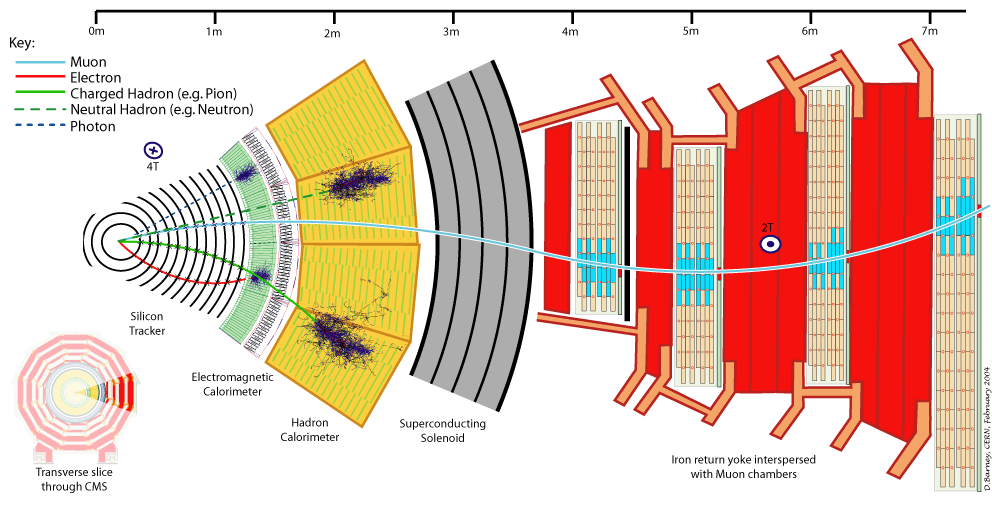
\includegraphics[width=0.9\linewidth]{Data/Introduction/CMS_layers.png}
\caption{A cross-sectional view of the CMS detection layers.}
\label{fig:cms_layers}
\end{figure}

The CMS detector consists of many separate detector layers, each of them playing an individual role in detecting and measuring the traversing particles. A cross-sectional overview of the layers and its tasks in reconstructing tracks of particles is shown in the Figure \ref{fig:cms_layers}.

\section{Phase II Upgrade of CMS Tracker}

After Phase II Upgrade, the LHC will provide a much higher luminosity. This regime is known as the High Luminosity LHC (HL-LHC). A serious problem presented by these conditions is the enormous data readout rates that exceed far beyond the bandwidth foreseen for the readout electronics.
However, the vast majority particles produced in the HL-LHC conditions are not of direct interest for new physics searches and are characterized by low transverse momentum. Thus rejecting tracker “hits” related to low transverse momentum particles can significantly reduce the amount of data to be readout. In order to provide momentum discrimination at the hardware level, a 2-layer module design was created. The central idea of the new modules is to provide fast discrimination between low and high transverse momentum particles by estimating the track curvature caused by the magnetic field within the volume of the module itself. For example, particle with high transverse momentum after hitting some pixel/strip at the first sensor layer would hit on of neighboring pixels/strips of the respective pixel/strip on the second layer. While a particle with low transverse momentum would have a more curved trajectory an hit pixel/strips at a displaced position from the first hit. By varying the distance between sensors and number of neighboring pixel/strips required to match hits in adjacent sensors, (2 neighboring strips in the Figure \ref{fig:low_high_pT}) it is possible to set the transverse momentum threshold for a hit~\cite{CMS_TECH_PHASE_II}.


\begin{figure}[ht]\centering
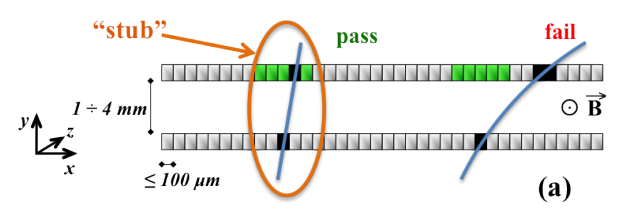
\includegraphics[width=0.8\linewidth]{Data/Introduction/Low_high_pT.png}
\caption{An example of distinguishing high and low transverse momentum. Particles, which hit any of two neighboring strips or the respective strip itself, would be record as high transverse momentum particles.}
\label{fig:low_high_pT}
\end{figure}


\textbf{Two layer Modules}

The CMS Phase-II Tracker will utilize two types of modules, 2S modules and PS modules. To achieve efficient rejection of low-pT (low transverse momentum) particles throughout the Tracker volume, modules in different regions will make use of a few different sensor spacings. For 2S (PS) modules, spacings of 1.8 and 4 mm (1.6, 2.6 and 4 mm) are foreseen. These modules will be used in the end-cap disks as well as the central barrel region of the Tracker. An exploded view of a PS module is shown in Figure \ref{fig:ps_exploaded}.
\begin{figure}[ht]\centering
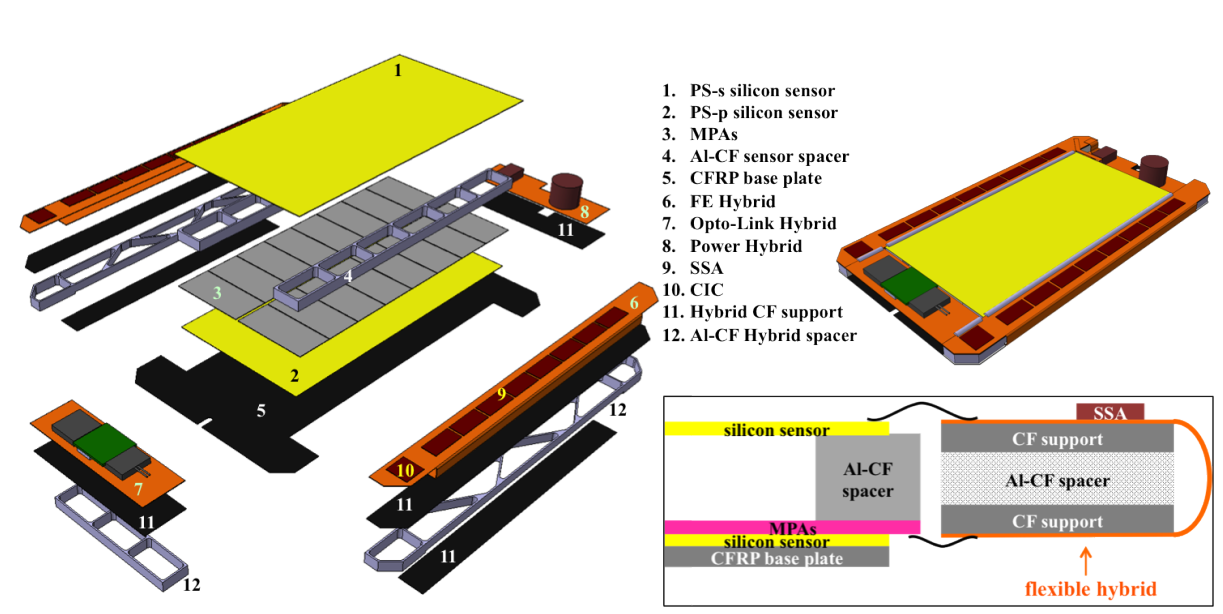
\includegraphics[width=0.8\linewidth]{Data/Introduction/PS_exploaded.png}
\caption{Exploaded view of Pixesl Sensor Module.}
\label{fig:ps_exploaded}
\end{figure}

In the PS module, the sensors are glued to a carbon-fibre reinforced Aluminium (AL-CF) spacers which act as spacers and provide the thermal conductance crucial for the cooling of the module. The two sensors and spacers are in turn glued the carbon-fibre (CF) baseplate. This structure is henceforth referred to as the sensor-spacer-baseplate-assembly (SSBA). This project will focus on the assembly of the SSBA only. The precision requirements of the SSBA are shown in Figure \ref{fig:ps(2s)_precision}. For the PS module, the sensors must align to within 40 mm measured at the sensor’s short edge. This corresponds to a rotational alignment tolerance of 0.8 mrad \cite{AutomatedAssembly_tutorial}.

\begin{figure}[ht]\centering
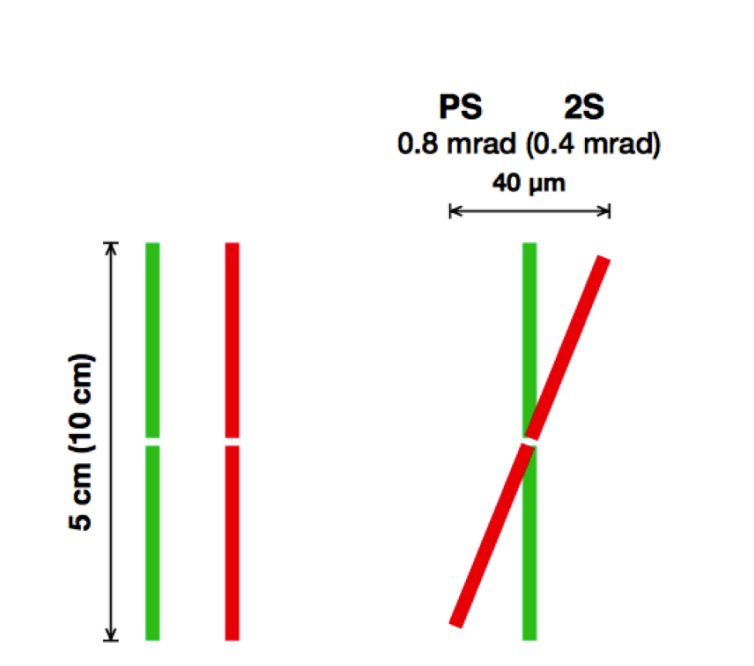
\includegraphics[width=0.4\linewidth]{Data/Introduction/PS(2S)_precision.png}
\caption{The precision requirements of the assembly of PS
and 2S modules.}
\label{fig:ps(2s)_precision}
\end{figure}
